\documentclass[a4paper,11pt]{article}

\usepackage{graphicx}
\usepackage[sort&compress]{natbib}
\usepackage{pdfpages}
\usepackage{amsmath}
\usepackage{breqn}
\usepackage{amssymb}
\usepackage{float}
\usepackage{listings}
\usepackage[a4paper]{geometry}
\usepackage{hhline}
\usepackage{makecell}

\begin{document}

\title{Research Project Proposal - Finding Interesting Patterns in Workflow Logging Data}
\date{\today}
\author{
        Dani\"el Stekelenburg, 4153286		
}
 
\maketitle

\abstract{}

\section{Introduction}
Optimizing the management of business processes becomes more and more important. Companies often use a software package which helps with collecting, storing and managing data from such processes. This category of software is called ERP, which stands for Enterprise Resource Planning. An example of ERP-software is the software-package \textit{Profit}, provided by a Dutch IT-company AFAS Software BV. For the experiment section, we will use the historical workflow logging data of Profit. The overall goal is to find interesting patterns in this data, such that we get a better understanding of what building blocks are mostly being used in workflows.

A technology for engineering business processes is workflow management. Although a workflow does not actually have a clear definition, we use the term \textit{workflow} to refer to an organized set of \textit{tasks} to accomplish some business process \cite{Georgakopoulos1995}. The basic idea of a workflow model is to capture dependencies between process tasks in a graph. For instance, when the graph contains a relation $A \rightarrow B$, this means that task $A$ generally precedes task $B$ in an instance of this workflow. Thus, task $B$ cannot be executed until task $A$ is finished. Workflow modeling makes the intended behavior or so-called flow of a business process clear and can be used to steer such processes into the right direction.\\
The goal of \textit{workflow mining} is to revert this process, meaning that we try to find a suitable workflow based on a given set of execution logs of a business process.

\subsection{A simple example}
To make things more concrete, let us use a graph-like structure to represent a workflow. See Figure \ref{figure:example_workflow} for a simple example. The workflow shows the process of buying additional leave, and consists of a set of tasks and a set of actions. One task is the starting point - in this case \textit{Buying additional leave} - and one action is the ending point (the rightmost \textit{Accept}). For every task, I added which person needs to complete that task in order for the workflow to progress. (1) An employee fills in an application for buying additional leave, (2) his manager needs to approve the request and (3) the administrator also needs to approve this. 

\begin{figure}[H]
\centering
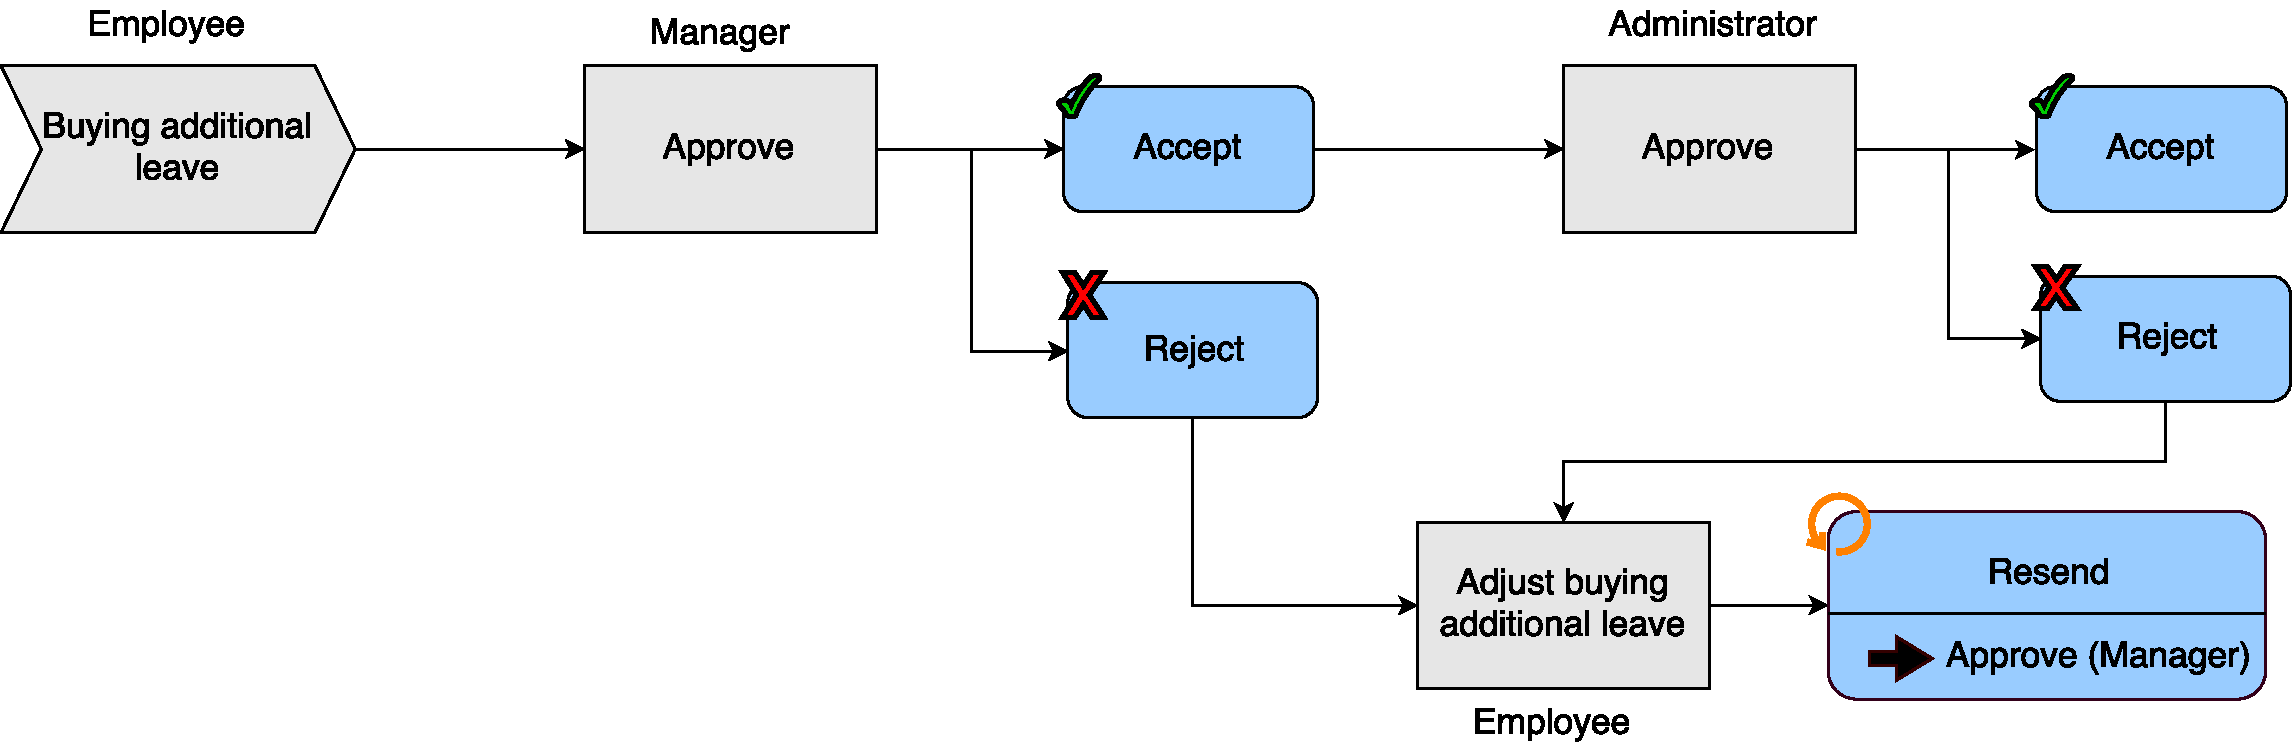
\includegraphics[width=\linewidth]{Example_Workflow.pdf}
\label{figure:example_workflow}
\caption{Example workflow, representing the process of buying additional leave. Gray nodes are tasks, whereas blue nodes are actions. }
\end{figure}

In case one of the two approvers does not agree with the request, the employee needs to adjust his request. Note that the action \textit{Resend} refers to the task \textit{Approve}. This means that this action leads to the task \textit{Approve} (another way to show this functionality would be to simply add an arrow from \textit{Resend} to the leftmost Approve\textit{Approve}). Finally, the workflow is completed when the rightmost \textit{Accept} action is executed.
\\
\\
Besides tasks and actions, there are workflow patterns. According to \cite{Riehle1996}, a pattern \textit{“is the abstraction from a concrete form which keeps recurring in specific nonarbitrary contexts”}. In other words, a pattern is an abstraction of a concrete set of tasks of actions and is independent of the workflow language used. An example is the or-split workflow pattern, which is visible in Figure \ref{figure:example_workflow}. Since the task \textit{Approve} has two actions and you may only choose one, you can see this structure as an OR-split (choose \textit{Okay} .

As a business company, you often can use workflows provided with your ERP-software package or create your own workflow. Provided workflow templates are in general workflows which represent very common business processes and most companies would like to use them. When you would like to have a workflow for a very specific process, you might have to assemble your own workflow structure.

In the eyes of an IT-company which develops and sells ERP-software, it is important to know which processes are most common in a company and what tasks are mostly used in workflows. Of course, having a good insight in the usage of workflows will be very helpful when you want to deliver a workflow management system. Getting a better understanding of the importance of a pattern in a workflow is the goal of this research project. More specifically, we try to find patterns in workflows which we classify as frequent.

This problem basically consists of the following subproblems:
\begin{enumerate}
\item What is a pattern?
\item When are two patterns equal?
\item When is a pattern frequent?
\item How can we mine occurrences of a pattern from a collection of logging data?
\end{enumerate}

\section{Literature Study}
This section refers to previous works, presenting valuable theories and techniques around workflows, patterns and the problem of mining such structures using workflow logs.

% Talk about process re-engineering in general and about workflows
Business process re-engineering is firstly proposed by \cite{Hammer1990} as an approach to tackle the problem of improving the quality of business processes, while reducing their cost. One of the earlier works presenting workflow management systems are \cite{EngelGLT79, Ellis1982}. The term \textit{information control net model} gets introduced by \cite{Ellis1982}, which can be seen as one of the earlier variants of workflow models. 

% Talk about workflow mining
Although the concept of process mining exists for over 25 years \cite{}, the paradigm of workflow mining is first introduced by \cite{Agrawal1998}. They present an algorithm which has a set of unstructured executions of a business process as input, and outputs a minimal dependency graph representing the control flow of this business process. 

% Talk about workflow patterns

% Talk about sequence mining

% Talk about word2vec




\bibliographystyle{unsrt}
\bibliography{sources}

\end{document}